% Copyright 2017 Emilio Rojas
%
% Permission is hereby granted, free of charge, to any person obtaining a copy of
% this software and associated documentation files (the "Software"), to deal in
% the Software without restriction, including without limitation the rights to
% use, copy, modify, merge, publish, distribute, sublicense, and/or sell copies of
% the Software, and to permit persons to whom the Software is furnished to do so,
% subject to the following conditions:
%
% The above copyright notice and this permission notice shall be included in all
% copies or substantial portions of the Software.
%
% THE SOFTWARE IS PROVIDED "AS IS", WITHOUT WARRANTY OF ANY KIND, EXPRESS OR
% IMPLIED, INCLUDING BUT NOT LIMITED TO THE WARRANTIES OF MERCHANTABILITY, FITNESS
% FOR A PARTICULAR PURPOSE AND NONINFRINGEMENT. IN NO EVENT SHALL THE AUTHORS OR
% COPYRIGHT HOLDERS BE LIABLE FOR ANY CLAIM, DAMAGES OR OTHER LIABILITY, WHETHER
% IN AN ACTION OF CONTRACT, TORT OR OTHERWISE, ARISING FROM, OUT OF OR IN
% CONNECTION WITH THE SOFTWARE OR THE USE OR OTHER DEALINGS IN THE SOFTWARE.

\textbf{Flip Flop $\text{J}_X$}
\begin{figure}[H]
  \centering
  \begin{subfigure}{0.1\textwidth}
    \centering
    \begin{tikzpicture}[scale=0.8]
      \draw(0,0) -- (0,0);
    \end{tikzpicture}
  \end{subfigure}
  \begin{subfigure}{.4\textwidth}
    \centering
    \begin{Karnaugh}{Y}{Z}{ZERO}{SP'}
      \minterms{14, 15}
      \implicant{15}{14}{blue}
    \end{Karnaugh}
  \end{subfigure}
  \begin{subfigure}{.4\textwidth}
    \centering
    \begin{Karnaugh}{Y}{Z}{ZERO}{SP'}
      \indeterminats{0, 1, 2, 3, 4, 5, 6, 7, 8, 9, 10, 11, 12, 13, 14, 15}
      \implicant{15}{14}{blue}
    \end{Karnaugh}
  \end{subfigure}

  \begin{subfigure}{0.5\textwidth}
    \centering
    \begin{tikzpicture}[scale=0.8]
      \draw(0,0) -- (0,0);
    \end{tikzpicture}
  \end{subfigure}
  \begin{subfigure}{.4\textwidth}
    \centering
    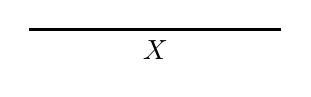
\begin{tikzpicture}[scale=0.8]
      \draw[very thick] (0,0.3) -- node [below]{$X$} ++(4,0);
    \end{tikzpicture}
  \end{subfigure}
  \caption*{$J_X = \color{blue} \text{Y} \cdot \text{Z} \cdot \text{ZERO}$.}
\end{figure}

\textbf{Flip Flop $\text{K}_X$}
\begin{figure}[H]
  \centering
  \begin{subfigure}{0.1\textwidth}
    \centering
    \begin{tikzpicture}[scale=0.8]
      \draw(0,0) -- (0,0);
    \end{tikzpicture}
  \end{subfigure}
  \begin{subfigure}{.4\textwidth}
    \centering
    \begin{Karnaugh}{Y}{Z}{ZERO}{SP'}
      \indeterminats{0, 1, 2, 3, 4, 5, 6, 7, 8, 9, 10, 11, 12, 13, 14, 15}
      \implicant{15}{14}{blue}
    \end{Karnaugh}
  \end{subfigure}
  \begin{subfigure}{.4\textwidth}
    \centering
    \begin{Karnaugh}{Y}{Z}{ZERO}{SP'}
      \minterms{14, 15}
      \implicant{15}{14}{blue}
    \end{Karnaugh}
  \end{subfigure}

  \begin{subfigure}{0.5\textwidth}
    \centering
    \begin{tikzpicture}[scale=0.8]
      \draw(0,0) -- (0,0);
    \end{tikzpicture}
  \end{subfigure}
  \begin{subfigure}{.4\textwidth}
    \centering
    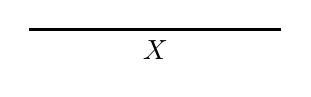
\begin{tikzpicture}[scale=0.8]
      \draw[very thick] (0,0.3) -- node [below]{$X$} ++(4,0);
    \end{tikzpicture}
  \end{subfigure}

  \caption*{$K_X = \color{blue} \text{Y} \cdot \text{Z} \cdot \text{ZERO}$.}
\end{figure}
